\documentclass[12pt,a4paper]{article}
\usepackage{textcomp,booktabs}
\usepackage{ctex}
\usepackage{amsmath,amscd,amsbsy,amssymb,latexsym,url,bm,amsthm}
\usepackage{epsfig,graphicx,subfigure}
\usepackage{enumitem,balance,mathtools}
\usepackage{wrapfig}
\usepackage{mathrsfs, euscript}
%\usepackage[usenames,dvipsnames]{color}
\usepackage{colortbl}
\usepackage{hyperref}
%\usepackage{picins}
\usepackage{extarrows}
\usepackage{float}
%\usepackage{algorithm}
%\usepackage{algorithmic}
%\usepackage[vlined,ruled,commentsnumbered,linesnumbered]{algorithm2e}
\usepackage[ruled,lined,boxed,linesnumbered]{algorithm2e}
\usepackage{textcomp,booktabs}

\definecolor{mygray}{gray}{.9}
\definecolor{mypink}{rgb}{.99,.91,.95}
\definecolor{mycyan}{cmyk}{.3,0,0,0}
\parindent=0pt
\parskip=3ex

\newtheorem{theorem}{Theorem}[section]
\newtheorem{lemma}[theorem]{Lemma}
\newtheorem{proposition}[theorem]{Proposition}
\newtheorem{corollary}[theorem]{Corollary}
\newtheorem{exercise}{Exercise}[section]
\newtheorem*{solution}{Solution}

\renewcommand{\thefootnote}{\fnsymbol{footnote}}

\newcommand{\postscript}[2]
 {\setlength{\epsfxsize}{#2\hsize}
  \centerline{\epsfbox{#1}}}

\renewcommand{\baselinestretch}{1.0}

\setlength{\oddsidemargin}{-0.365in}
\setlength{\evensidemargin}{-0.365in}
\setlength{\topmargin}{-0.3in}
\setlength{\headheight}{0in}
\setlength{\headsep}{0in}
\setlength{\textheight}{10.1in}
\setlength{\textwidth}{7in}
\makeatletter \renewenvironment{proof}[1][Proof] {\par\pushQED{\qed}\normalfont\topsep6\p@\@plus6\p@\relax\trivlist\item[\hskip\labelsep\bfseries#1\@addpunct{.}]\ignorespaces}{\popQED\endtrivlist\@endpefalse} \makeatother
\makeatletter
\renewenvironment{solution}[1][Solution] {\par\pushQED{\qed}\normalfont\topsep6\p@\@plus6\p@\relax\trivlist\item[\hskip\labelsep\bfseries#1\@addpunct{.}]\ignorespaces}{\popQED\endtrivlist\@endpefalse} \makeatother
\begin{document}
\noindent

%========================================================================
\noindent\framebox[\linewidth]{\shortstack[c]{
\Large{\textbf{Homework Syntax Analysis1}}\vspace{1mm}\\
Exercises for Complier Principles by Li Jiang, 2015 Autumn Semester}}
\begin{center}
\footnotesize{\color{blue} \quad Name:Qinyun Song  \quad Student ID:5120309059 \quad Email: haibara502@gmail.com}
\end{center}
\begin{enumerate}
% Problem One
\item Consider the context-free grammar:$S -> S S + | S S * | a$\\
and the string aa + a*. \\
a) Give a leftmost derivation for the string. \\
b) Give a rightmost derivation for the string. \\
c) Give a parse tree for the string. \\

\begin{solution}
	$   $
	\begin{enumerate}
		\item 
		\begin{displaymath}
			S \xLongrightarrow[lm]{} SS* \xLongrightarrow[lm]{} SS+S* \xLongrightarrow[lm]{} aS+S* \xLongrightarrow[lm]{} aa+S* \xLongrightarrow[lm]{} aa+a*
		\end{displaymath}
		
		\item
		\begin{displaymath}
			S \xLongrightarrow[rm]{} SS* \xLongrightarrow[rm]{} Sa* \xLongrightarrow[rm]{} SS+a* \xLongrightarrow[rm]{} Sa+a* \xLongrightarrow[rm]{} aa+a*
		\end{displaymath}
		
		\item
		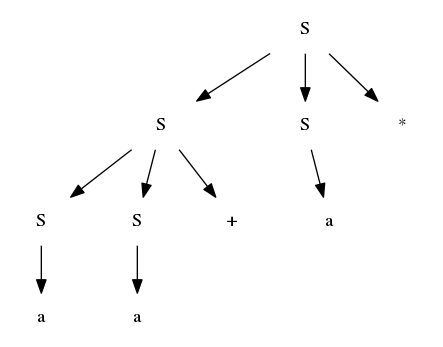
\includegraphics[width=0.5\textwidth]{parseTree.png}
	\end{enumerate}
\end{solution}

%problem two
% Problem One
\item The following is a grammar for regular expressions over symbols a and b only, using + in place of j for union, to avoid conflict with the use
of vertical bar as a metasymbol in grammars:\\
$$rexpr -> rexpr + rterm | rterm$$
$$rterm -> rterm rfactor | rfactor$$
$$rfactor -> rfactor * | rprimary$$
$$rprimary -> a | b$$
a) Left factor this grammar.\\
b) Does left factoring make the grammar suitable for top-down parsing?\\
c) In addition to left factoring, eliminate left recursion from the original grammar.\\
d) Is the resulting grammar suitable for top-down parsing?\\

\begin{solution}
	$   $
	\begin{enumerate}
		\item This grammar is already left factored. \\
		\item No. \\
		\item 
		$$rexpr \to rterm \; rexpr'$$
		$$rexpr' \to +rterm \; rexpr' | \epsilon$$
		$$rterm \to rfactor \; rterm'$$
		$$rterm' \to rfactor \; rterm' | \epsilon$$
 		$$rfactor \to rprimary \; rfactor' $$
		$$rfactor' \to *rfactor' | \epsilon $$
		$$rprimary \to a | b $$
		\item Yes.
	\end{enumerate}
\end{solution}

%problem Three
\item Compute FIRST and FOLLOW for the grammar:\\
a) $S -> 0 S 1 | 0 1 with string 000111$.\\
b) $S -> + S S | * S S | a with string + * aaa$.\\

\begin{solution}
	$   $
	\begin{enumerate}
		\item 
		FIRST(S) = \{0\} \\
		FOLLOW(S) = \{1, \$\} \\
		\item
		FIRST(S) = \{+, *, a\}\\
		FOLLOW(S) = \{+, *, a, \$\}
	\end{enumerate}
\end{solution}
\end{enumerate}
%========================================================================
\end{document}
